\chapter{Обзор существующей проблемы}\label{ch:overview:1}

\section{Обзор современного состояния и ключевых проблем проектирования, потенциальных решений для конструкций резервуаров для хранения криогенного жидкого водорода для применения в авиации}\label{ch:overview:1:sec1}
% https://ntrs.nasa.gov/api/citations/20060056194/downloads/20060056194.pdf

\subsection{Абстракт}\label{ch:overview:1:sec1:sub1}

Благодаря высокой удельной энергоемкости жидкий водород (\(LH_2\) --- liquid hydrogen~\(H_2\)) выделяется на горизонте альтернативных источников энергии для будущих летательных аппаратов. Как следствие, существует потребность в системах хранения водорода, которые должны обеспечивать достаточную вместимость для полетов продолжительностью от нескольких минут до нескольких дней. Понятно, что разработка большого, легкого, многоразового криогенного резервуара для хранения водорода имеет решающее значение для достижения целей и обеспечения топливом летательных аппаратов на водороде, особенно для длительных полетов. В данной работе  представлен обзор текущего состояния дел в области материалов, конструкций и систем изоляции криогенных резервуаров ---- наряду с попыткой определения ключевых проблем  разработки легкой и долговременной системы хранения \(LH_2\). Рассмотренные широкие классы изоляционных систем включают пенопласты (включая современные аэрогели) и системы многослойной изоляции (МСИ -- MLI --- multilayer insulation) с вакуумом. Системы МСИ показывают перспективность для долгосрочного применения. Рассмотренные структурные конфигурации включают одно- и двустенные конструкции, в том числе многослойные конструкции. Потенциальными кандидатами для материала стенок являются монолитные металлы, а также полимерные матричные композиты и прерывисто армированные металлические матричные композиты. Для применения в кратковременных полетах может быть достаточно простых конструкций баков. В качестве альтернативы для более длительных полетов наиболее оптимальной представляется конструкция с двойными стенками и вакуумной системой изоляции. Современные тенденции в разработке материалов для обшивки рассматриваются в случае, когда обшивка требуется для минимизации или устранения потерь водородного топлива через проницаемость.


Интерес к разработке летательных аппаратов, использующих альтернативные источники энергии, такие как водород, обусловлен прежде всего тем, что водород обеспечивает низкий или нулевой выброс в окружающую среду вредных продуктов. Среди рассматриваемых вариантов применения -- продолжительность полета, которая может составлять от нескольких минут до многих дней. Как пример, вот пример современного беспилотного летательного аппарата (БПЛА)  NASA с большой продолжительностью полета: Helios~HP03, БПЛА на солнечных батареях, использующий систему регенеративных топливных элементов для накопления энергии. Он был способен летать в течение месяца, но имел ограниченную грузоподъемность 230 кг (550 фунтов), которая должна была распределяться по крыльям, и мог летать на пиковой высоте около 21 км (70 000 футов).

В коммерческих самолетах продолжительность полета, скорее всего, будет составлять порядка нескольких часов. Стремление к увеличению грузоподъемности и продолжительности полета требует использования силовой установки с более высокой удельной мощностью и повышенной общей эффективностью. Исследуемые в настоящее время системы включают использование топливных элементов с электродвигателями и двигателями внутреннего сгорания. Текущие предварительные требования к программам, которые стимулируют разработку водородных самолетов с большой продолжительностью полета, включают продолжительность полета 14 дней (336 часов) с полезной нагрузкой, достаточной для размещения приборов.

Водород обладает наибольшей энергией на единицу массы среди различных видов жидкого и газообразного топлива, как отмечает Томас (\cite{thomas2000}). Водород, хранящийся в жидком виде, значительно увеличивает энергию на единицу объема по сравнению с газообразным водородом (\(GH_2\) --- gaseous hydrogen). Газообразный водород, хранящийся при давлении 35~МПа~(5~ksi) и температуре \(20^{\circ} C \,(68^{\circ} F)\), хранит только одну треть энергетического содержания на единицу объема жидкого водорода (\(LH_2\)), как показано Томасом. Хотя для хранения (\(LH_2\)) при низком давлении и криогенной температуре требуется изоляция, она меньше, чем при хранении  (\(GH_2\)) при высоком давлении. Другой метод хранения водорода в компактной и безопасной форме --- это гидрид металла. К сожалению, использование гидридов металлов накладывает ограничение, связанное с чрезмерным весом, что исключает их использование в чувствительных к весу приложениях. 

В настоящее время применение криогенных резервуаров для хранения в аэрокосмической отрасли, где вес имеет первостепенное значение, ограничено короткими полетами, например, на космических ракетах-носителях. 
Криогенные жидкости переливаются в баки для хранения транспортного средства непосредственно перед запуском, а большая часть жидкостей расходуется во время выхода на орбиту, в течение нескольких минут. 
Криогенные жидкости исчерпываются со скоростью, при которой выкипание не представляет значительной проблемы (\( {\color{red} \text{уточнить у кого-нибудь, кто в теме}} \)). В таких случаях для резервуаров обычно достаточно легкой пенопластовой изоляции. 
В глубоком космосе теплопередача к криогенной жидкости значительно меньше, чем в условиях окружающей среды на поверхности Земли, что снижает необходимость в сверхнизкой проводимости и толстой изоляции. Именно для самолетов с относительно большой продолжительностью полета порядка нескольких дней возникают наибольшие инженерные трудности при разработке долговременных и легких систем хранения водорода.

Необходимость снижения веса в сочетании с хорошими изоляционными свойствами для долгосрочного хранения представляет собой новую задачу в проектировании криогенных резервуаров. Это дает возможность применить более современные материалы и конструктивные идеи в попытке снизить общий вес и сохранить объем на приемлемом и практичном уровне.

В данном работе рассматриваются конструктивные и тепловые элементы системы баков для хранения криогенных веществ для летательного аппарата. В следующих разделах будут рассмотрены отдельные компоненты системы баков. 

После подробного описания основных проблем в следующих разделах будут рассмотрены подкомпоненты системы баков. Также будут рассмотрены материалы и их термическая и химическая совместимость со средами, в которых работает система хранения \(LH_2\). Будут рассмотрены методы строительства резервуара. Сюда входит оценка металлических и полимерно-матричных композитных (ПМК) материалов и архитектуры, используемой для создания резервуара. Также будет обсуждаться возможность использования футеровки ({\color{green}  Футеровка (нем. Futter «подкладка, подбой») -- облицовка огнеупорными, химически стойкими, износостойкими, а также теплоизоляционными материалами, которым покрывается внутренняя поверхность металлургических печей, ковшей, топок котлов и прочего оборудования. Футеровка производится для обеспечения защиты поверхностей от возможных механических, термических, физических и химических повреждений.}).

Другие важные области конструкции бака, включая методы крепления для интеграции системы бака с планерной рамой, ребра жесткости, перегородки для выброса топлива и порты, подробно не рассматриваются, поскольку они выходят за рамки данного отчета.

Методы изоляции будут рассмотрены для определения оптимальной системы для применения в летательных аппаратах. 

\section{Ключевые проблемы разработки}\label{ch:overview:1:sec2}

Успешная реализация будущих легко-весных и экологически чистых ЛА требует объединения ряда инновационных и передовых технологий, а также разработки новых технических средств и технологий их производства. Как уже упоминалось выше, особый интерес представляют ЛА на водородном топливе с продолжительностью полета в несколько дней. Водород можно хранить как в газообразной, так и в жидкой форме. Газообразный водород требует в \(5.6\) раз большего объема по сравнению с жидкой форме, при этом жидкий водород хранится под давлением примерно \(163\) атм (\(2400\) фунтов на кв. дюйм) и при температуре \(15^{\circ}C (60^{\circ}F)\).

Необходимый при этом чрезмерный объём, вес бака и проблемы связанные с обеспечением безопасности, при с хранением водорода под высоким давлением, исключают использование газообразного водорода \(GH_2\) в качестве топлива для данного применения. В качестве альтернативы, гидриды металлов могут компактно и безопасно хранить водород, хотя эти системы будут слишком тяжелыми и, следовательно, непрактичными. Кроме того, для <<перезарядки>> большинства металлогидридных систем потребуются дни или даже недели. Гидриды \(MgNi\) могут достичь приблизительно 5 процентов водорода по весу, но требуют более высоких температур для активации кристаллического слоя.

Проблемы металлогидридов были обобщены Брюером (\cite{brewer1991}), который отметил их непрактичность для авиационных применений. Жидкий водород в насыщенном состоянии является жизнеспособным вариантом для самолетов с большой продолжительностью полета. Однако проектирование криогенного резервуара для хранения \(LH_2\), в сочетании с использованием \(LH_2\) в качестве авиационного топлива, сопряжено со многими проблемами. Некоторые из ключевых проблем, включая геометрию, температуру, проницаемость, водородное охрупчивание и факторы безопасности, кратко обсуждаются ниже.

\subsection{Реальные размеры, геометрия}\label{ch:overview:1:sec2:sub1}

Несмотря на то, что жидкий водород \(LH_2\) имеет высокую температуру сгорания, его низкая плотность в сочетании с потенциально большой продолжительностью полета и использованием нерекуперативной системы хранения может привести к необходимости бака большого объема.

Неинтегральный (т.е. не являющийся частью конструкции летательного аппарата) большой бак означает большую лобовую (поперечную) площадь и площадь поверхности, что приведет к увеличению сопротивления. Для успешных конфигураций потребуются инновационные конструкции с малой лобовой площадью и площадью поверхности.

Интеграция большого бака в ЛА сама по себе является серьезной проблемой. Интегральные баки, напротив, требуют сложной конструкции и создают множество производственных проблем. Интегральные баки являются конструктивным элементом ЛА, т.е. воспринимают нагрузки на фюзеляж, а также обеспечивают сохранность топлива. Неинтегральные баки служат только в качестве контейнеров для топлива и устанавливаются внутри корпуса ЛА и удерживаются им (\cite{brewer1991}). Как упоминалось ранее, неинтегральные баки не обязательно должны соответствовать форме ЛА; их конструкция может быть относительно простой, например, сферической или цилиндрической. Баки сферической формы обеспечивают минимальную площадь поверхности для данного объема, поэтому пассивное нагревание бака может быть сведено к минимуму, что минимизирует выкипание LH2. Однако сферическая форма создает некоторые специфические производственные трудности и имеет большую площадь фронтальной поверхности, что приводит к увеличению силы сопротивления по сравнению с баком цилиндрической формы. В качестве альтернативы, цилиндрические формы проще в изготовлении, но имеют более высокое отношение площади поверхности к объему, что приводит к более высокой пассивной тепловой нагрузке на бак.

\subsection{Криогенные температуры}\label{ch:overview:1:sec2:sub2}

Нормальная температура кипения \(LH_2\) составляет \(-252^{\circ}C (-423^{\circ}F)\). \(LH_2\) необходимо держать ниже этой температуры, чтобы минимизировать выкипание, то есть потерю топлива и повышение давления в баке. Во время наземных операций максимальная разница температур внутри и снаружи конструкции бака может достигать \(\Delta T = 300^{\circ}C~(540^{\circ}F)\). Для поддержания такого большого температурного градиента, очевидно, необходима легковесная изоляция с низкой теплопроводимостью. Как уже упоминалось, большинство предыдущих применений криогенного топлива, такого как \(LH_2\), было ограничено короткой продолжительностью в несколько минут, как в ракетах-носителях, где проблема выкипания топлива не является критической. Однако для полетов большой продолжительности чрезмерное выкипание топлива очень нежелательно и ограничивает продолжительность полета летательного аппарата. Следовательно, количество пассивного тепла, которое поступает в бак и вызывает выкипание жидкого водорода, должно быть ограничено. Хранение \(LH_2\) на земле имеет аналогичные проблемы и требует специализированного оборудования и процедур для работы с ним. Установлено, что если поддерживать постоянное абсолютное давление \(LH_2\) на уровне примерно \(170 кПа (25 psia)\), то выкипание будет поддерживаться на приемлемом уровне и без лишних весовых нагрузок на конструкцию резервуара (\cite{brewer1991}). Кроме того, резервуар и любые соединительные трубопроводы или приспособления должны быть полностью изолированы от внешней атмосферы, поскольку все газы, за исключением гелия, застывают при температурах LH2 и повышают вероятность образования закупорки проточных трубопроводов и других компонентов.

\subsection{Проницаемость}\label{ch:overview:1:sec2:sub3}

Поскольку молекулы водорода очень малы, они чрезвычайно легко проникают через стенку резервуара. Проницаемость водорода является, пожалуй, самым критическим моментом в конструкции резервуара. Металлические баки являются очевидным решением этой проблемы, поскольку водород проникает через металлы медленнее, чем сквозь неметаллические материалы. Однако для летательного аппарата масса металлического бака может ограничить его грузоподъемность и продолжительность полета. Бак из композита с полимерной матрицей (КПМ --- PMC polymer matrix composite) с тонкой металлической обшивкой также решил бы проблему проницаемости, но вес все еще может оказаться проблемой. Кроме того, несоответствие коэффициента теплового расширения (КТР) между стенкой композитного бака и металлическим вкладышем приведет к их неравномерному сжатию, что, в результате, может вызвать напряжения в материале, которые могут привести к отслойке вкладыша от бака и/или его разрушению, что делает такую конструкцию нежелательной. 

Исследования проницаемости водорода, проведенные в ходе программы "Национальный аэрокосмический самолет" ( National Aerospace Plane program), были обнадеживающими, и было показано, что композитные баки без какого-либо вкладыша достаточно непроницаемы. Однако разрушение бака КПМ \(LH_2\) демонстрационного проекта X-33 во время наземных испытаний было вызвано микротрещинами полимерной матрицы в композитной внутренней оболочке конструкции бака (\cite{grimsley2001}). Микротрещины в композите возникли в результате несоответствия КТР углеродного волокна и полимерной матрицы в сочетании с большой разницей между температурой использования и температурой изготовления композита. Микротрещины создавали путь для утечки или проникновения водорода под давлением через стенку и проникновения в сотовый заполнитель. При нагревании трещины в матрице закрывались, жидкость испарялась, а образовавшиеся газы, которым некуда было выходить, вызывали повышение давления и в конечном итоге отслоение сердечника от внутренней композитной оболочки.  В последнее время были проведены исследования по оценке полимерных пленок и покрытий, которые можно было бы нанести на внутреннюю композитную оболочку и использовать в качестве барьера для удержания \(LH_2\) в резервуаре. Изготовление легких и непроницаемых резервуаров из современных материалов для криогенного применения является сложной задачей.

\subsection{Водородное охрупчивание}\label{ch:overview:1:sec2:sub4}

Многие материалы при воздействии водорода в больших концентрациях становятся хрупкими. Влияние водорода на поведение материалов хорошо описано (например, \cite{moodythompson1990}). Это один из видов разрушения материала. Когда материал становится более хрупким, его несущая способность и пластичность снижаются. Таким образом, могут произойти катастрофические разрушения без значительной деформации или видимого деградирования детали конструкции. Это ограничивает применение многих современных материалов в строительстве стенки резервуара.

Для решения этих проблем необходимы прорывные технологии в области материалов. Для возникновения водородного охрупчивания необходимы растягивающие напряжения, восприимчивый к воздействию водорода материал и присутствие водорода. Водородное охрупчивание может привести к образованию трещин при уровнях напряжения значительно ниже предела текучести. Хотя водородное охрупчивание больше всего зафиксировано для высокопрочных сталей, все материалы обладают определенной степенью восприимчивости. Устойчивость к водородному охрупчиванию должна быть важным фактором при выборе материалов для стенок резервуара.

\subsection{Коэффициент безопасности}\label{ch:overview:1:sec2:sub5}

Использование требуемых коэффициентов безопасности в диапазоне от \(1.4\) до \(2.0\), которые обычно дополняются консервативными расчетами на прочность материала (такими как использования допустимых значений на основе А-базиса), очень затрудняет достижение облегченной конструкции. Это особенно актуально, когда в строительстве таких конструкций используются нетрадиционные передовые материалы. Кроме того, новые и/или современные материалы не очень хорошо изучены, особенно при экстремально низких температурах, а процессы производства и изготовления вносят дополнительную вариативность в свойства материала. Все это приводит к значительному разбросу свойств материалов, что требует значительной разницы между средними измеренными и допустимыми значениями.

Будущие конструкции резервуаров, безусловно, потребуют инновационных разработок, выверенных с помощью испытаний и включающих интегрированные методы мониторинга состояния здоровья для снижения явных и неявных коэффициентов безопасности.  В целом, поиск правильного баланса между (1) минимизацией веса прочной конструкции бака, вмещающей необходимое количество топлива, (2) выживанием в течение необходимого количества циклов полета, включающих циклы заправки и слива топлива и соответствующие термомеханические нагрузки, и (3) созданием конструкции, которая может быть действительно изготовлена, проверена и использована с уверенностью.


\section{Предыдущий опыт использования креогенных баков}\label{ch:overview:1:sec3}

Исследования в области хранения \(LH_2\) для летательных аппаратов и космических кораблей проводились в течение многих лет. Поскольку летательные аппараты и космические аппараты имеют схожие требования, ниже приводится краткий обзор прошлых разработок криогенных баков для авиакосмической техники в хронологическом порядке. Также приводится краткое описание других применений, включая мобильные и стационарные наземные хранилища. 

\subsection{Самолеты с водородными двигателями на заре авиации}\label{ch:overview:1:sec3:sub1}

Одно из самых ранних задокументированных примеров использования криогенного резервуара для хранения водорода и заправки водородным топливом летательного аппарата было представлено Холом и Сильверштейном (\cite{hallsilverstein1955}) и Рейнольдсом (\cite{reynolds1955}). Двухмоторный бомбардировщик ВВС США B-57 был модифицирован таким образом, чтобы один из двигателей работал на водороде. Это было частью программы Исследовательского центра НАСА имени Гленна (NASA Glenn Research Center), Кливленд, штат Огайо (бывший Исследовательский центр Льюиса), для демонстрации характеристик сгорания водорода в авиационных газотурбинных установках, как отмечает Брюер (\cite{brewer1991}). Следует отметить, что основной упор в программе был сделан на успешную работу газотурбинного двигателя на водороде; следовательно, не было уделено внимание разработке легкой системы криогенных резервуаров.


\subsection{Сатурн 5. <<Saturn V>>}\label{ch:overview:1:sec3:sub2}

Ракета Saturn V --- американская сверхтяжёлая ракета-носитель семейства Сатурн, использовавшеяся в 1960-х и 1970-х годах. В ракете Saturn V использовались алюминиевые баки с пенопластовой изоляцией. Одностенный металлический бак с изоляцией из пенопласта достаточно показателен для типичных ракетоносителей, использующих жидкий водород в качестве топлива для запуска с Земли на орбиту. То, что ракета-носитель была запущена с Земли на орбиту, обуславливает такое хранение как краткосрочное.

Две верхние ступени двигателя Saturn V использовали \(LH_2\) вместе с жидким кислородом (\(LO_2\)) в качестве топлива. Глейзер (\cite{glaser1967}) показал вторую ступень, состоящую из алюминиевой стенки, окруженной сотовым заполнителем из пенопласта, затем нейлоновым фенольным покрытием и последним слоем пластиковой пленки Tedlar (DuPont) для защиты от аэродинамического нагрева. Пенопласт продувался гелием. Глейзер описал третий этап как использование пенопласта на внутренней стороне стенки резервуара. Расположение пенопласта уменьшило необходимость в специальных методах и клеях для крепления пенопласта. В результате стенка бака работала при более высокой температуре и не нуждалась в защите от аэродинамического нагрева. На внутренней поверхности изоляции был установлен паро- и жидкостный барьеры.

\subsection{Внешний бак космического челнока. <<Space Shuttle>>}\label{ch:overview:1:sec3:sub3}

С начала 1980-х годов и по настоящее время НАСА использует космический челнок в качестве тяжелого ракето-носителя. Внешний бак космического челнока (ВБ) представляет собой современную легкую конструкцию криогенного хранилища, которая используется в настоящее время. Внешний бак является несущей конструкцией в системе космического челнока. Он предназначен для хранения \(LH_2\) и \(LO_2\), нагрузки от самого орбитального корабля и нагрузки от твердотопливных ракетных ускорителей (боковой ускоритель, SRB ---  solid rocket boosters). Кроме того,  криогенные жидкости хранятся под давлением около 2 атм. Внешний бак --- это расходуемый компонент, который заполняется непосредственно перед запуском и используется в течение короткого промежутка времени при выведении шаттла со стартовой площадки на низкую околоземную орбиту примерно за \(8.5\)~мин. Вес хранимого \(LH_2\) составляет \(1.0\) МН (228 000 фунтов) со скоростью выкипания примерно \(4.4\) Н/с (1 фунт/с) при стабилизации бака (П. Роджерс, 2006, NASA Marshall Space Flight Center, Huntsville, AL, личное сообщение), что соответствует примерно \(1.6\,\%\) от веса \(LH_2\) в час.  Часть внешнего бака, находящаяся под давлением, изготовлена из алюминиево-литиевого сплава 2195. Первоначально использовался алюминиевый сплав 2219, который позже был заменен на алюминиево-литиевый сплав 2195, как описано Бикли и Швингхамером (\cite{bickleyschwinghame1999}). Алюминиево-литиевый сплав обеспечивает увеличение прочности и небольшое снижение плотности по сравнению с ранее использовавшимся сплавом 2219.  ВБ представляет собой алюминиевую полумонококовую конструкцию из сваренных плавлением стволовых секций, пяти основных кольцевых рам, а также носового и кормового эллипсоидных куполов, согласно Petty (\cite{petty2006}). Тепловая защита обеспечивается напыляемой пеной и предварительно формованными материалами абляторов. На веб-сайте НАСА, посвященном ВБ, Петти дает хороший обзор бака.


\subsection{X-30 National Aero-Space Plane. <<NASP>>}\label{ch:overview:1:sec3:sub4}

Совместные усилия Министерства обороны США (МО) и НАСА по разработке Национального аэрокосмического самолета (NASP) в течение большей части 1980-х годов включали попытку разработать легкие криогенные баки для одноступенчатого аппарата для полета с Земли на орбиту. Некоторые из усилий NASP были обобщены в работах Cope и Thorndyke (\cite{copethorndyke1992}) и Hellwig et al. (\cite{hellwig1992}). Изначально NASP был исследованием целесообразности создания одноступенчатого транспортного средства, способного взлетать и приземляться горизонтально, как кратко описано в работе Jenkins et al. (\cite{jenkins2003}). Потенциальный прототип получил обозначение X-30. Позднее рамки программы были изменены для разработки гиперзвукового межконтинентального самолета. 

Жесткие требования, предъявляемые к одноступенчатым и гиперзвуковым межконтинентальным аэрокосмическим аппаратам, повышали важность снижения веса. В проекте NASP использовался многослойный композитный бак для хранения жидкого водорода. Это была ранняя попытка использования КПМ с криогенными жидкостями для снижения веса по сравнению с более распространенными металлическими конструкциями. Бак был изготовлен из тонкостенного композита с эпоксидной матрицей, армированного углеродным волокном, с элементами жесткости, как описано в Hellwig et al. (\cite{hellwig1992}). Кроме того, в баке использовались внутренние ограничители для уменьшения деформации стенок бака при нагнетании давления (\cite{lohmuelle2006}) и отсутствовала обшивка (\cite{robinson1994}).

\subsection{Первый летательный аппарат, работающий только на водороде}\label{ch:overview:1:sec3:sub5}

Брюер (\cite{brewer1991}) описал первый самолет, полностью работающий на водородном топливе. Полет состоялся 19 июня 1988 года. Предыдущие самолеты использовали несколько двигателей, и только один двигатель работал на водороде. В самолете, описанном Брюером, для хранения LH2 использовался цилиндрический бак с эллипсоидными торцевыми крышками. Бак был изготовлен из нержавеющей стали типа 304. Емкость была установлена внутри алюминиевого внешнего корпуса и опиралась в нескольких точках на распорки с низкой теплопроводностью. Пространство между баком и оболочкой было вакуумировано для минимизации теплопроводности, а для минимизации радиационной теплопередачи внутри вакуумированного пространства использовалась многослойная изоляция. Однако общая цель программы заключалась в демонстрации полета с использованием исключительно двигателя на водородном топливе, а не в разработке легкого бака для хранения LH2 в течение длительного времени. 

\subsection{Lockheed Martin X-33}\label{ch:overview:1:sec3:sub6}

Проект X-33 был естественным продолжением проекта NASP (Х-30). Программа NASA X-33 была важным проектом, в котором использовались передовые материалы и концепции для усовершенствования технологии криогенных баков-аккумуляторов. Суборбитальный корабль Х-33 был разработан для демонстрации передовых технологий, которые должны были значительно повысить надежность ракеты-носителя и снизить стоимость выведения полезной нагрузки на низкую околоземную орбиту. X-33 должен был стать средством демонстрации технологий для VentureStar. Большая часть работы над X-33 была обобщена в отчете Центра космических полетов НАСА имени Джорджа К. Маршалла (\cite{nasamarshall2000}).

На аппарате X-33 было два топливных бака LH2, каждый размером 8,7 на 6,1 на 4,3 м (28,5 на 20 на 14 футов). Исследования водородной проницаемости, проведенные в ходе программы NASP, были обнадеживающими, и считалось, что композитные баки без какого-либо вкладыша достаточно непроницаемы. На Х-33 использовалась более сложная трехслойная сендвич-конструкция баков. Многослойная конструкция состояла из графит-эпоксидных внутренней и внешней обшивок и графит-эпоксидного невентилируемого сердечника Hexcel Composites, как описано в Dornheim (\cite{dornheim1999}). Баки состояли из трех основных субкомпонентов: кормового купола и переборки, стволовой секции и носового купола и переборки. Баки также являлись неотъемлемой структурной частью основного корпуса корабля и должны были находиться в очень сложном напряженном состоянии. Эти баки были испытаны в Центре космических полетов имени Маршалла НАСА в Хантсвилле, штат Алабама, в ноябре 1999 года для проверки структурной целостности баков LH2 при криогенной температуре и различных условиях давления и механических нагрузок, предполагаемых как типичные для использования в аппарате Х-33.

После успешного завершения первого испытания прототипа на давление и нагрузку, из испытуемого изделия был слит LH2 и началась продувка бака. Примерно через 15 минут после слива жидкости из бака произошла авария: внешняя лицевая панель и сердцевина одной из долей отделились от внутренней лицевой панели. Было установлено, что все процедуры испытания и параметры находились в пределах конструктивных ограничений испытуемого изделия.

Была собрана следственная группа, которая назвала наиболее вероятной причиной отказа сочетание следующих явлений (отчет NASA Marshall, \cite{nasamarshall2000}):  (1) Микротрещины во внутреннем слое лицевой панели с последующей просачиванием жидкого водорода (2) Попадание внешнего азотистого газа в вакуум и последующее разжижение при контакте с криогенной границей (3) Снижение предела прочности и жесткости клеевой линии (4) Производственные браки и дефекты (5) Просачивание жидкого водорода в наполнитель панели, что привело к более высокому, чем ожидалось, давлению в сотовой панели.

Последний фактор стал неожиданной причиной возникновения разрушения. Конструкция бака расширила границы возможностей  и объединила множество непроверенных технологических элементов, создав очень сложную систему. Использование замкнутого композитного бака не только для перевозки топлива, но и для передачи механических нагрузок было довольно смелым решением для того времени. Процесс производства выявил некоторые сложности, связанные с масштабированием больших композитных конструкций, которые не были изучены ранее. Главным уроком, извлеченным из этого опыта, стало явление и значение микротрещин в композитных панелях криогенных баков под воздействием тепловых и механических нагрузок. Отказ испытательного аппарата X-33 во время наземных испытаний был обобщен в работе Grimsley et al. (\cite{grimsley2001}), которая показала, что причиной отказа стало проникновение водорода в сердцевину композитной многослойной структуры через микротрещины матрицы.


Тем не менее, группа по расследованию аварий (отчет NASA Marshall, \cite{nasamarshall2000}) отметила, что результаты исследования не опровергают использование композитных материалов для криогенных баков. 


Уроки, извлеченные из этого испытания, если их применить к технологии композитных криогенных баков с точки зрения проектирования и производства, должны способствовать развитию технологии и успешному использованию композитов для будущих криогенных баков. 

 Ближе к концу программы было принято решение продолжить использование водородного бака из алюминиевого сплава для испытательного аппарата X-33 после того, как возникли трудности с баком КПМ. Программа X-33 выявила те области, которые требуют дальнейшего изучения и развития, включая решение проблемы микротрещинообразования композитов, использование вкладышей и других деталей конструкции стенок бака.

\subsection{Резервуар для жидкого водорода в программе Next Generation Launch Technology}\label{ch:overview:1:sec3:sub7}

Программа Next Generation Launch Technology (NGLT) была продолжением программы X-33 по разработке следующего поколения многоразовых аэрокосмических аппаратов. Программа NGLT основывалась на опыте X\nobreakdash-33. Предварительный анализ концепции бака был выполнен Абумери и др. (\cite{abumeri2004}) в рамках программы NASA NGLT. Концепция конструкции состояла из бака КПМ с тонкими стенками и дополнительными внутренними слоями ламината, образующими продольные ребра жесткости. Другое исследование Робинсона и др. (\cite{robinson2004}) иллюстрировало исследования по определению конструкции бака для следующей многоразовой ракеты-носителя. Результаты этих исследований привели к созданию композитного бака из углеродного волокна с сотовым сердечником и многослойной структурой, используемой на X-33 и в проекте NGLT. После проведения дополнительных исследований в рамках проекта NGLT была введена защитная пленка на внутренней стенке бака.

В продолжение проекта криогенного бака X-33 NASA и Northrop Grumman разработали и завершили испытания уменьшенного композитного криогенного бака в Marshall. Эти баки были ключевым частью всех многоразовых элементов программы NASA NGLT. Эти баки также были составной частью планера; то есть они несли стартовые нагрузки и нагрузки на крыло в дополнение к топливу. Четвертьмасштабный цилиндрический бак длиной 4,6 м (15 футов) и диаметром 1,8 м (6 футов) был опрессован под давлением около 779 кПа (113 фунтов на кв. дюйм).

Это тестовое давление примерно в четыре раза превышает эксплутационное давление в реальном полноразмерном баке, чтобы вызвать аналогичные напряжения стенок, возникающие при запуске из-за нагрузок от жидкости, ускорения и т.д. Согласно планам испытаний, бак должен был быть охлажден, наполнен и подвергнут нагрузке около 40 раз в течение нескольких месяцев (Glass, \cite{glass2004}, и Sharke, \cite{sharke2004}). Согласно пресс-релизу подрядчика NASA - компании Northrop Grumman - эти испытания были успешно завершены (McKinney and Neiwert, \cite{mckinneyneiwert2004}).

\subsection{Другие сферы применения криогенных хранилищ}\label{ch:overview:1:sec3:sub8}

В настоящее время ведутся исследования по созданию недорогих легких криогенных хранилищ для наземного транспорта. Наземные транспортные средства имеют требования к долгосрочному хранению, аналогичные тем, которые необходимы для гражданских самолетов. Министерство энергетики США (DOE) уже давно работает с водородом в качестве топлива для транспортных систем. Одна из попыток включала создание автомобиля, работающего на LH2, как представил Стюарт (\cite{stewart1982}). В этой работе использовался бак-накопитель более традиционной конструкции, то есть металлический бак с изоляцией MLI. Масса системы является важным вопросом для наземного транспорта, такого как автомобили, но не в такой степени, как для воздушных и космических транспортных средств. Общая стоимость, как правило, является значительной движущей силой наряду с требованиями к малому весу.

Другие автомобильные проекты кратко описаны в DaimlerChrysler (\cite{daimlerchrysle2004}). Пример автомобильного криогенного бака представлен Magna Steyr (\cite{magnasteyr2006}), который является частью совместных усилий BMW AG, Linde AG и Magna Steyr и состоит из двустенного бака, изготовленного из аустенитной стали. В объеме между стенками используется MLI и поддерживается высокий вакуум 10-9 бар. Это похоже на ранний проект DOE, представленный Стюартом (\cite{stewart1982}).

Стационарные наземные хранилища не имеют строгих ограничений по весу и размеру, налагаемых подвижными системами. Таким образом, такие резервуары также могут быть изготовлены из аустенитной стали, окруженной вакуумной защитной оболочкой с MLI. Кроме того, для долгосрочного хранения можно использовать холодильную установку. Однако системы баков для хранения водорода, используемые в самолетах, требуют использования чрезвычайно легких конструкций. Необходимость создания легких, хорошо изолированных систем хранения, пригодных для полетов, представляет собой настоящую инженерную задачу. 

Следует отметить, что многие исследования и разработки, включая NASP, X-33 и NGLT, проводились для приложений, требующих относительно короткой продолжительности работы. Короткая продолжительность позволяет увеличить потери из-за утечек и выкипания по сравнению с длительной продолжительностью полета водородного самолета. Многие из вышеупомянутых вариантов применения сфокусированы на силовых установках, работающих на водороде. В результате в опубликованных отчетах были представлены минимальные подробности структурных конструкций систем хранения, используемых в этих приложениях. Хотя вышеупомянутые программы ракет-носителей продвинули вперед технологию легких криогенных баков-аккумуляторов, все еще существует необходимость в разработке системы изоляции бака, которая была бы легкой и способной удерживать утечку и выкипание на приемлемом уровне. 


\section{Возможные пути решения}\label{ch:overview:1:sec4}

Как обсуждалось ранее, соответствующая система теплоизоляции имеет важнейшее значение для резервуаров для хранения LH2, особенно для длительных режимов эксплуатации. Экономичная и легкая система теплоизоляции минимизирует выкипание LH2, при этом минимально увеличивая общую массу конструкции резервуара. Еще одна функция изоляции является предотвращение конденсации и последующего застывания атмосферных газов на баке. 

Эта задача может быть решена путем использования либо системы с вакуумной оболочкой, либо системы с продувкой (такой как с гелиевой продувкой), где воздух заменен неконденсирующимся газом. Поддержание адекватного уровня вакуума является одной из основных трудностей при использовании системы с вакуумной оболочкой и, конечно же, становится все труднее по мере того, как более высокий уровень вакуума требуется для поддержания теплофизических свойств. Дополнительным фактором является способность изоляционной системы выдерживать изменения размеров из-за наложенных термических циклов нагружения в результате заполнения криогенным (охлажденным) водородом. Следовательно, несоответствие КТР между компонентами системы резервуара является ключевым фактором. При проектировании резервуарной системы необходимо оценить влияние, связанные с несоответствием КТР компонентов резервуарной системы. 

Кроме того, механическое сжатие изоляционной системы может произойти из-за собственного веса, перепада давления, внешних ударов и вибрации, изменения размеров или любой комбинации этих нагрузок и снизить ее эффективность.  Считается, что изоляционная система имеет низкое контактное сопротивление, если ее теплопроводность чувствительна к нагрузке на сжатие. Наконец, желательно, чтобы изоляционная система и ее основные компоненты обладали низкой теплопроводностью и низкой массовой плотностью. Считается, чтоТакже желательно, чтобы коэффициент радиационной теплопередачи был низким.


\subsection{Учёт тепловой нагрузки: Изоляция}\label{ch:overview:1:sec4:sub1}

Как уже говорилось ранее, соответствующая система теплоизоляции имеет решающее значение для резервуаров для хранения жидкого водорода, особенно для длительных операций. Эффективная и легкая система изоляции сводит к минимуму выкипание LH2 при минимальной массе общей конструкции резервуара. Еще одна функция изоляции - предотвращение конденсации и последующего застывания атмосферных газов на резервуаре. 
Это можно преодолеть, используя либо систему с вакуумной оболочкой, либо продуваемую систему (такую как 
с гелиевой продувкой), где воздух заменен неконденсирующимся газом. Поддержание адекватного уровня вакуума 
является одной из основных трудностей при использовании системы с вакуумной оболочкой и, конечно же, становится все сложнее, так как более высокие значения вакуума требуются для поддержания тепловых свойств. Дополнительным моментом является способность изоляционной системы выдерживать изменения размеров из-за наложенных термических циклов в результате 
заполнения криогенным водородом. Следовательно, несоответствие КТР между компонентами системы резервуара является ключевым фактором. При проектировании резервуарной системы необходимо оценить проблемы, связанные с несоответствием КТР 
 При проектировании резервуарной системы необходимо оценить вопросы, связанные с несоответствием КТР между компонентами стенок резервуара должны быть оценены и учтены при проектировании. Кроме того, механическое сжатие изоляционной системы может произойти из-за веса, перепада давления через изоляции, ударов и вибрации, изменения размеров или любой комбинации этих нагрузок и снизить ее эффективность.  эффективность. Считается, что изоляционная система имеет низкое контактное сопротивление, если ее теплопроводность 
чувствительна к нагрузке на сжатие. Наконец, желательно, чтобы изоляционная система и ее основные И наконец, желательно, чтобы изоляционная система и ее основные компоненты обладали низкой теплопроводностью, а также низкой теплопроводностью и низкой массовой плотностью. Также желательно, чтобы коэффициент радиационной теплопередачи был низким. 

Построение диаграмм свойств материала, позволяюют оценить тепловые и механические показатели эффективности,  позволят разработать эффективную схему изоляции для длительных продолжительных полетов. Как отмечалось ранее, показатели эффективности могут помочь сузить круг возможных вариантов выбора инженерных материалов и систем для изоляционной системы для долговременного легкого криогенного хранилища жидкости. хранения. На \cref{fig:figure4} показан график зависимости теплопроводности от массовой плотности, так как низкий вес для применения в летательных аппаратах имеет решающее значение. Для долгосрочного применения низкая теплопроводность чрезвычайно важна. Изоляционные схемы, в которых используются такие материалы, как полимерные пены низкой плотности, включая новые материалы типа аэрогеля, являются желательными, как видно из \cref{fig:figure4}. Комбинация вакуумной оболочки и многослойной изоляции имеет диапазон плотностей, сравнимый с пенопластами низкой плотности, и относительную теплопроводность, которая примерно на два порядка ниже, чем у лучших пенопластов низкой проводимости (за пределами диапазона, представленного на \cref{fig:figure4}).
\begin{figure}[h!]
\centering
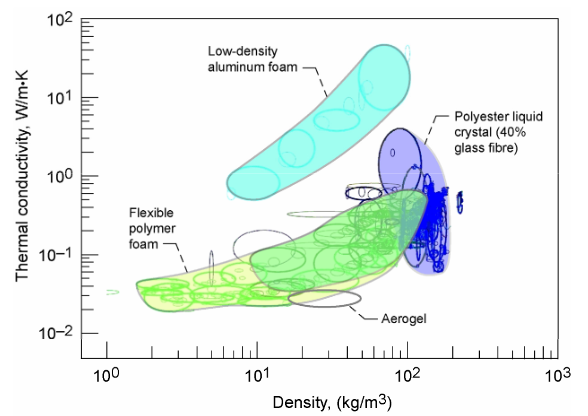
\includegraphics[width=0.75\textwidth]{figure4.png}%

\caption{Отношение термопроводности к удельной плотности для разнообразных инженерных материалов (взято из \cite{ashby2005})}
\label{fig:figure4}
\end{figure}


На \cref{fig:figure5} показан график зависимости теплопроводности (thermal conductivity) от температуропроводности (thermal diffusivity) для различных материалов. Многослойная изоляция имеет тепловую диффузию, сравнимую с семейством металлов, но явную теплопроводность примерно на два порядка ниже, чем у полимерных пен. Для заданной толщины изоляции, следует выбирать систему с наименьшей теплопроводностью, чтобы минимизировать установившийся теплового потока и низкой теплопроводностью, то есть высокой удельной теплоемкостью, чтобы максимизировать время, необходимое для того, чтобы тепловой энергии для достижения криогенной жидкости. Следующее уравнение связывает время достижения устойчивого состояния, \(t\), с толщиной стенки, \(w\), и температуропроводностью, \(a\).
Для заданной толщины стенки желательно минимизировать теплопроводность, чтобы максимизировать время, необходимое для достижения устойчивого состояния, особенно для кратковременных применений. Минимизация отношения \(k/a^{\frac{1}{2}}\), где k - теплопроводность, приводит к максимизации энергии, запасенной в материале для данной дельты температуры и времени. Это максимизирует время, затрачиваемое на то, чтобы тепло могло хранить криогенной жидкости без изменений. 
\[t=\frac{w^2}{2a}\]

\begin{adjustwidth}{3.5em}{3.5em}
{\color{green} Минутка ВИКИПЕДИИ.

Теплопроводность материала (thermal conductivity) --- это мера способности материала проводить тепло через себя. температуропроводность материала (thermal diffusivity), с другой стороны, является тепловой инерцией этого материала.


В физике теплопроводность --- это способность материала проводить тепло. Теплопроводность обозначается символом K. Единицей измерения теплопроводности в СИ является ватт на метр Кельвина (Вт/мК). Теплопроводность данного материала часто зависит от температуры и даже от направления теплопередачи. Согласно второму закону термодинамики, тепло всегда течет от горячей области к холодной. Другими словами, для чистого переноса тепла необходим градиент температуры. Чем выше теплопроводность материала, тем выше скорость передачи тепла через этот материал. 


Температуропроводность (коэффициент температуропроводности) --- физическая величина, характеризующая скорость изменения (выравнивания) температуры вещества в неравновесных тепловых процессах. Численно равна отношению теплопроводности к удельной теплоёмкости при постоянном давлении.  Ее можно понимать как способность материала проводить тепло относительно тепла, аккумулированного в единице объема. Это означает, что чем выше теплопроводность, тем выше температуропроводность.  Температуропроводность газа очень чувствительна к температуре, а также к давлению. Единицей измерения теплопроводности в СИ является м2с-1.
}
\end{adjustwidth}

\begin{figure}[h!]
\centering
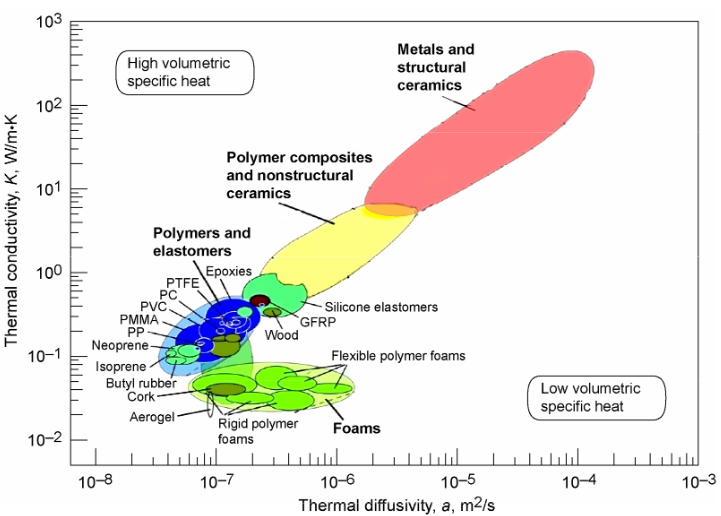
\includegraphics[width=0.75\textwidth]{figure5.png}%
\caption{Отношение теплопроводности от температурапроводности для разнообразных материалов  (взято из \cite{ashby2005}). GFRP -- стеклопластик, PC--- поликарбон, PMMA -- полиметилметакрилат (органическое стекло), PP -- полупропилен, PTFE -- тефлон и PVC -- поливинилхлорид}
\label{fig:figure5}
\end{figure}

На \cref{fig:figure6} показана зависимость теплопроводности от коэффициента теплового расширения для различных материалов. Также на рисунок добавлен примерный режим работы аэрогеля, основанный на данных M.A. Meador (\cite{meador2005}, Исследовательский центр Гленна, Кливленд, штат Огайо, личное сообщение). Этот график полезен для оценки теплового искажения. Значение \(\frac{k}{\alpha}\), где \(\alpha\) -- КТР, может быть использовано в качестве показатель термического искажения. Материалы с большим значением этого показателя демонстрируют небольшое термическое искажение.


Изоляционные материалы по своей функциональности, имея низкие значения теплопроводности, показывают большие тепловые градиенты и, следовательно, высокие тепловые искажения.  Таким образом, материалы с низкой теплопроводностью и, кроме того, обладающие низким КТР, являются желательными. Высокое тепловое искажение может привести к сравнительно большому относительному перемещению, которое может вызвать напряжение в изоляционном материале, превышающее его прочность. прочность материала. Механическое разрушение может привести к ухудшению тепловых свойств изоляционной системы. После выбора класса материалов на основе их тепловых характеристик следует использовать материалы с наименьшим значением \(\alpha\), чтобы минимизировать тепловое искажение и вызванные им напряжения.

Низкая теплопроводность является важным свойством для любой изоляционной системы, особенно для долгосрочного применения. В результате, из \cref{fig:figure6} видно, что жесткие полимерные пенопласты, включая аэрогели, являются жизнеспособной изоляционной системой, поскольку они обеспечивают низкую теплопроводность. Аэрогели в этой группе, по-видимому, имеют более низкий КТР. Как показано на \cref{fig:figure6}, металлические материалы обладают более низким КТР, что приводит к меньшим искажениям; однако их более высокая теплопроводность (и плотность) не позволяет рассматривать их в качестве изоляционных материалов.

\begin{figure}[h!]
\centering
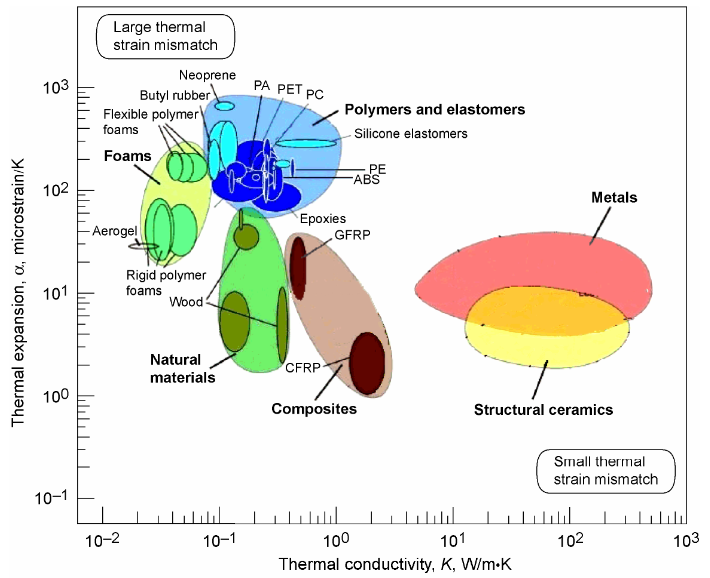
\includegraphics[width=0.75\textwidth]{figure6.png}%
\caption{Отношение КТР от теплопроводности для разнообразных материалов  (взято из \cite{ashby2005}). ABS -- АБС-пластик, GFRP -- стеклопластик, PC--- поликарбон, PMMA -- полиметилметакрилат (органическое стекло), PP -- полупропилен, PTFE -- тефлон и PVC -- поливинилхлорид}
\label{fig:figure6}
\end{figure}

Диапазон значений теплопроводности различных материалов обусловлен уровнем вакуума и разницей температур. Например, системы МСИ обеспечивают очень низкие значения относительной теплопроводности порядка \(10^{-6} \text{Вт/м} \cdot \text{K} (6\times10^{-7} \text{БТу/фут}\cdot \text{час}^{\circ}F)\).
В системах МСИ используется несколько экранов теплового излучения, расположенных перпендикулярно направлению теплового потока. Радиационные экраны представляют собой чередующиеся слои металлической фольги с низкой излучательной способностью (обычно алюминизированный майлар (DuPont)) и тонкая изолирующая прокладка (обычно полиэстер или стекловолоконная бумага), соединенные таким образом, чтобы исключить контакт металла с металлом. Однако существуют строгие требования, которые необходимо учитывать при выборе системы МСИ. Главным требованием к системе МСИ является поддержание уровня вакуума ниже 13 МПа , чтобы система МСИ сохраняла свою эффективность. Теплопередача за счет остаточной газопроводности происходит в условиях пониженного вакуума. Перфорационные отверстия в слоях майлара очень важны для обеспечения отвода остаточных газов при установке вакуумной изоляции и/или системы МСИ. Кроме того, его тепловые свойства сильно анизотропны и чувствительны к механическому сжатию (низкое контактное сопротивление).  Система МСИ была впервые запатентована Матшем (\cite{matsch1961}).

Последние достижения в области МСИ для криогенных резервуаров для хранения включают разработку МСИ с переменной плотностью (МСИПП), где расстояние между слоями варьируется в поперечном сечении МСИ. Радиационная теплопередача обычно преобладает в более теплых внешних слоях стандартной системы МСИ, в то время как теплопроводность играет большую роль в более холодных внутренних слоях. За счет большего расстояния между внутренними слоями уменьшается как масса МСИПП, так и тепловые утечки. Недавно Гастингс и др. (\cite{hastings2004}) провели испытания гибридной системы изоляции из напыляемой пены (SOFI) и МСИПП для орбитального применения. Эта система спроектирована таким образом, чтобы полагаться на SOFI при высоком давлении во время наземного удержания и запуска и на МСИ во время орбиты. 45-слойное одеяло МСИПП варьировалось от 8 слоев/см (20 слоев/дюйм.) в холодной области до 16 слоев/см (41 слой/дюйм.) в теплой области. Испытания показали, что по сравнению со стандартным МСИ с 70 равномерно распределенными слоями уменьшилось выкипание на 41 процент.


Другой предложенной системой изоляции была изоляция микросферами, которая состоит из полых стеклянных сфер различного диаметра и толщины стенок. Она не так чувствительна к условиям вакуума, как МСИ, а также обеспечивает некоторую структурную поддержку с минимальным увеличением низкой теплопроводности при сжимающих нагрузках. Влияние двух промежуточных газов, азота и гелия, при различных давлениях на относительную теплопроводность микросферной изоляции было экспериментально оценено и соотнесено с аналитическими моделями Каннингтоном и Тьеном (\cite{cunnington1978}). Дальнейшие усилия Пармли и Каннингтона (\cite{parmleycunnington1979}) позволили получить данные для проектирования гибкой системы микросферной изоляции из нержавеющей стали в вакуумной оболочке. Современные разработки включают производство автономных эвакуированных изоляционных панелей из микросфер, заключенных в гибкую вакуумную барьерную пленку (Allen et al., \cite{allen2004}). Эти панели обладают теплопроводностью, составляющей примерно половину теплопроводности пенополиуретана.


Другой класс материалов, которые рассматриваются для криоизоляции, -- аэрогель кремнезема. Аэрогели кремнезема -- это твердые вещества с высокой пористостью и очень низкой плотностью, состоящие из взаимосвязанных частиц, которые образуют "открытую" микроструктуру. Теплопроводность аэрогелей кремнезема, как правило, очень низкая, обычно менее \(40\times10^{-3} \text{Вт/м} \cdot K (23 \cdot 10^{-3} \text{БТу/фут} \cdot \text{час}\cdot ^{\circ}F) \), что обусловлено очень низкой теплопроводностью кремнезема, а также размерами пор, которые составляют порядка нанометров. Чрезвычайно низкая теплопроводность делает аэрогели кремнезема очень востребованными для широкого спектра изоляционных применений. Однако те же свойства аэрогелей, которые делают их чрезвычайно хорошими изоляторами -- высокая пористость и низкая плотность -- также делают их по своей природе хрупкими и ломкими. Таким образом, их использование в несущих нагрузку приложениях (таких как криогенные резервуары для хранения LH2 для полетов) является проблематичным. В настоящее время ведутся исследования по улучшению механических свойств аэрогелей без чрезмерного ущерба для их других уникальных свойств. Однако
признано, что любое улучшение механических свойств происходит за счет увеличения плотности массы и, следовательно, увеличения веса и теплопроводности. Один из подходов, использованных Каннингтоном, Ли и Уайтом (1997), заключается в создании композитов волокно/аэрогель путем добавления небольшой объемной доли (менее 5 процентов) коротких волокон кремнезема или карбида кремния. Волокна уменьшают прозрачность для теплового излучения при температурах выше температуры окружающей среды, тем самым увеличивая тепловые характеристики. Волокна также укрепляют аэрогель. Однако этот подход имеет значение только тогда, когда излучение является основным способом передачи тепла, по сравнению с твердофазным и газофазным способами теплопроводности, которые возникают при температурах выше 27 °C (80 °F) и 127 °C (260 °F) соответственно. В Исследовательском центре НАСА имени Гленна также ведутся работы по созданию аэрогелей из сшитого кремнезема, модифицированных эпоксидными смолами для получения механически прочного, но легкого пористого материала (Meador et al., 2005, и Leventis et al., 2003).


\subsection{Возможные материалы и особенности конструкции резервуаров}\label{ch:overview:1:sec4:sub2}

Хранение жидкого водорода в легком резервуаре само по себе представляет значительные трудности. Более низкая плотность водородного топлива приводит к необходимости использования емкости большего объема по сравнению с другими видами топлива. Механические нагрузки на бак определяются (1) разницей между давлением внутри бака и окружающей средой, (2) весом топлива, (3) ускорением транспортного средства, (4) проскальзыванием топлива при маневрах самолета и (5) весом системы бака и его опор. При маневрировании летательного аппарата или при столкновении с воздушной турбулентностью во время полета обязательно возникнет всплеск/бултыхание топлива.

Для поддержания водорода в жидком состоянии необходимо поддерживать постоянное абсолютное давление во внутреннем резервуаре. Давление также будет способствовать перекачке водорода из бака к силовой установки. Холл и Сильверштейн (\cite{hallsilverstein1955}) предположили, что 2 атм (200 кПа, 29 psi) будет достаточно для перекачки топлива в крейсерском режиме для летательного аппарата. Петти (2002) также подтвердил, что внешний бак космического челнока работает в диапазоне давлений 220-230 кПа (32-34 psi), что близко к диапазону, предложенному Холлом и Сильверстайном. Кроме того, с увеличением рабочего давления увеличивается проектный вес бака. Поэтому крайне желательно поддерживать давление в резервуаре как можно более низким, как отметил Рейнольдс (\cite{reynolds1955}). Как правило, газообранзый водород используется в качестве нагнетателя для жидкого водорода.

Два важных критерия для стенки резервуара включают выбор материала и конструкции стенки. Существует множество вариантов, и они обсуждаются в следующих разделах. Обсуждаются преимущества и недостатки различных вариантов, а также даются рекомендации по выбору оптимальной системы.

\subsubsection{Выбор материала стенки резервуара}\label{ch:overview:1:sec4:sub2:subsub1}

Очевидно, что желательно использовать материалы, обладающие высокой прочностью, высокой вязкостью разрушения и высокой жесткостью, а также низкой плотностью и низкой проницаемостью для жидкого и газообразного водорода; однако ни один материал не обеспечивает все эти свойства одновременно.
Следовательно, показатели характеристик материала связаны с этими свойствами. Среди этих параметров прочность и плотность имеют большую значимость для расчета. На \cref{fig:figure7} показана зависимость прочности от массовой плотности для различных инженерных материалов. В данном случае предпочтительными являются материалы, расположенные в левом верхнем углу.
Композитные материалы обладают высокой удельной прочностью по сравнению с металлами и вполне подходят для аэрокосмических применений. В частности, из \cref{fig:figure7} видно, что композиты из полимеров, армированных непрерывным волокном (CFRP, углепластик), обеспечивают самую высокую прочность и при этом являются наиболее легкими. Однако использование композитных материалов, армированных непрерывным волокном, скорее всего, повлечет за собой более высокие первоначальные производственные затраты. Согласно \cref{fig:figure7}, материалами, обладающими достаточной прочностью и приемлемой низкой плотностью, являются КПМ и металлические материалы.
материалы. Керамические материалы также обладают высокой удельной прочностью, но из-за низкой вязкости разрушения они не подходят для использования в качестве материала стенки резервуара.

Потенциальной более дешевой альтернативой композитам, армированным непрерывным волокном, могут быть металлические композиты с дискретным армированием (КДА), в частности, дискретно армированный алюминий (ДАА), описанный Miracle (\cite{miracle2005}). ДАА являются по существу изотропными и могут быть изготовлены с использованием менее дорогостоящих технологий, таких как литье. На \cref{fig:figure8} показан удельный модуль упругости относительно удельной прочности. На этом рисунке желательно использовать материалы, расположенные ближе к правому верхнему углу. Материалы КДА хорошо сопоставляются с композитными материалами на основе полимеров. Дополнительным преимуществом материалов КДА является чрезвычайно низкая (если не пренебрежимо малая) газопроницаемость водорода, обычно связанная с композитными системами на основе полимерных матриц.


\begin{figure}[h!]
\centering
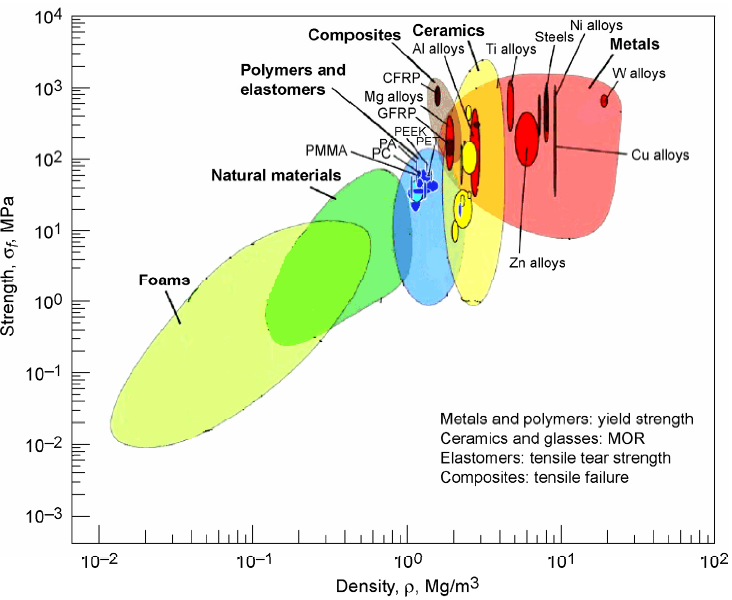
\includegraphics[width=0.75\textwidth]{figure7.png}%
\caption{Отношение прочности к массовой плотности для разнообразных материалов  (взято из \cite{ashby2005}). CFRP -- углепластик, GFRP -- стеклопластик, PA --- полианилин. PC--- поликарбон, PEEK --- полиэфирэфиркетон, PET --- полиэтилен ,PMMA -- полиметилметакрилат (органическое стекло)}
\label{fig:figure7}
\end{figure}

\begin{figure}[h!]
\centering
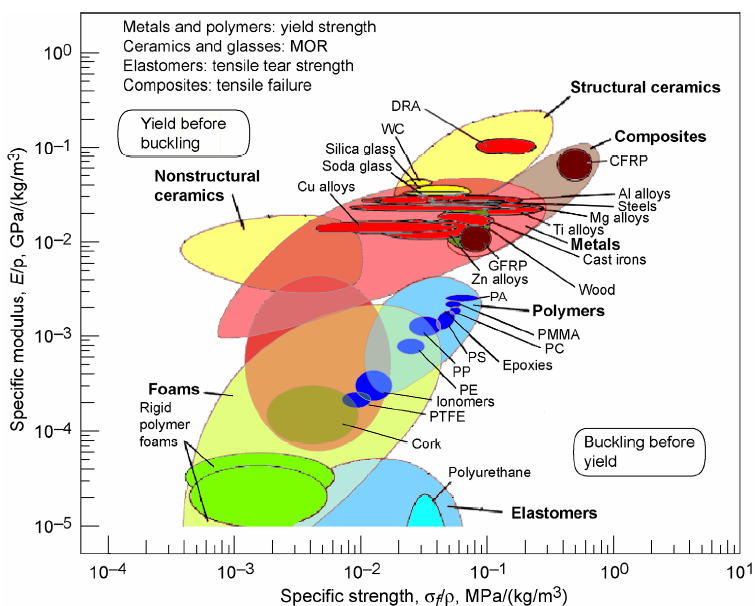
\includegraphics[width=0.75\textwidth]{figure8.png}%
\caption{Отношение удельной модуль упругости от удельной прочности для разнообразных материалов  (взято из \cite{ashby2005}). CFRP -- углепластик, DRA -- дискретно-армированный алюминий, GFRP -- стеклопластик, PA --- полианилин. PC--- поликарбон, PE --- полиэтилен ,PMMA -- полиметилметакрилат (органическое стекло)}
\label{fig:figure8}
\end{figure}

Ключевыми свойствами материала, которые важны для проектирования сосудов высокого давления, но также могут быть применимы к криогенным резервуарам низкого давления, являются <<текучесть до разрушения>>, \(K_{Ic}/\sigma_f\), и <<утечка до разрушения>>, \(K_{Ic}2/\sigma_f\). Они могут быть получены из \cref{fig:figure9}, где \(K_{Ic}\) -- вязкость разрушения, а \(\sigma_f\) -- прочность материала. Использование первого показателя гарантирует, что напряжение, необходимое для распространения критического дефекта, будет больше, чем напряжение, необходимое для деформации материала. Таким образом, сосуд будет стабильно деформироваться таким образом, чтобы его можно было обнаружить. Второй критерий, используемый в основном для больших сосудов, гарантирует, что максимальное давление приведет к стабильному росту трещины, достаточно большой для проникновения как во внутреннюю, так и во внешнюю поверхность, так что утечка может быть обнаружена до катастрофического разрушения. Заметим, что оба показателя могут быть максимизированы, уменьшая предел текучести самой стенки, однако это может не только ограничить способность сосуда выдерживать давление, но и привести к чрезмерно большой толщине стенок и, следовательно, к очень тяжелому резервуару. Толщина стенки резервуара \(t\) определяется следующим уравнением для тонкостенных сферических резервуаров: 

\[t \geq \frac{pR}{2 \sigma_f}\]

где \(p\) -- давление в резервуаре, \(R\) -- радиус резервуара, а \(\sigma_f\) -- прочность материала резервуара, как показано на \cref{fig:figure8}. Чтобы минимизировать массу резервуара и понимая, что масса резервуара прямо пропорциональна толщине стенки резервуара, желательно выбрать такой материал для стенки резервуара, который максимизирует удельную предельную прочность.

\begin{figure}[h!]
\centering
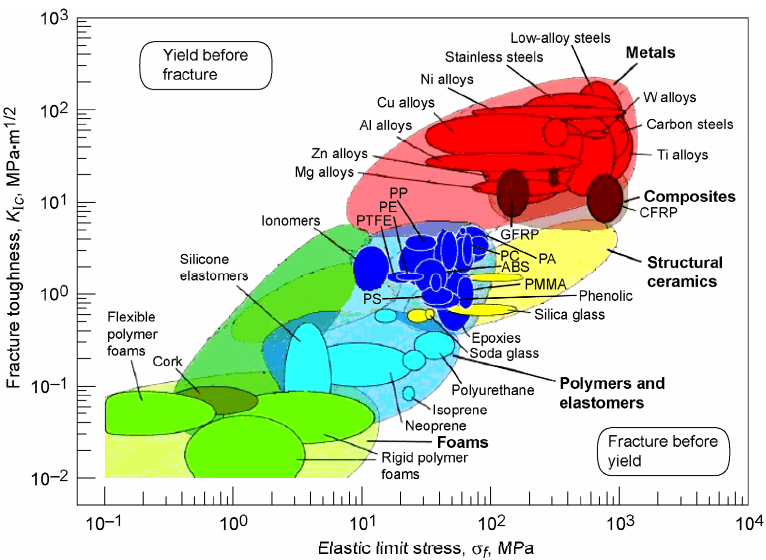
\includegraphics[width=0.75\textwidth]{figure9.png}%
\caption{Отношение вязкости разрушения от прочности для разнообразных материалов  (взято из \cite{ashby2005}). CFRP -- углепластик, DRA -- дискретно-армированный алюминий, GFRP -- стеклопластик, PA --- полианилин. PC--- поликарбон, PE --- полиэтилен, PMMA -- полиметилметакрилат (органическое стекло)}
\label{fig:figure9}
\end{figure}

Рассмотрим следующие параметры материала 
\[ M_1 = \frac{\rho}{\sigma_f} \]
\[ M_2 = \frac{\rho}{K_{Ic}} \]

Первый индекс \(M_1\) основан на требовании, чтобы прочность материала стенки не была превышена, в то время как второй индекс материала \(M_2\) основан на требовании, чтобы вязкость разрушения материала не была превышена. Масса тонкостенного сферического резервуара с радиусом \(R\) и толщиной стенки \(t\) определяющаюся как
\[ m = \left (\pi c \right)^{1/2} M_2 \]

Действующее напряжение в баке от действия внутреннего давления
\[ \sigma = \frac{p R}{2 t}\]

Минимизирую массу резервуара с учетом показанных параметров выше, объеденяя оба параметра, получим
\[ M_1 = \left ( \pi c \right ) ^{1/2} M_2\]
где \(c\) критический размер трещины для данного материала.

На \cref{fig:figure10} показан соответствующий график с двумя линиями связи, соответствующими длинам трещин 5 мм и 5 мкм. Это показывает, что выбор материала может быть ограничен способностью обнаруживать трещины заданного размера. Например, выбор материала будет ограничивается монолитными металлическими сплавами, если можно обнаружить только трещины размером более 5 мм. Однако, как показано на \cref{fig:figure10}, другие материалы, включая керамику и эластомеры, могут быть жизнеспособными материалами, если трещины размером 5 мкм
или больше могут быть обнаружены.

\begin{figure}[h!]
\centering
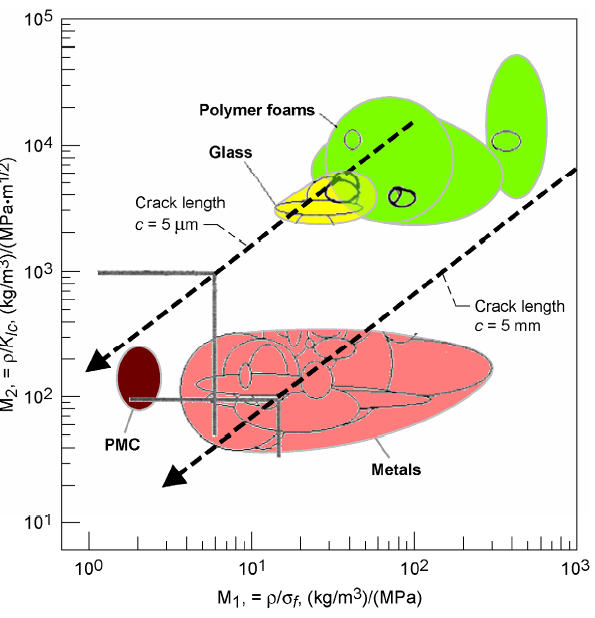
\includegraphics[width=0.75\textwidth]{figure10.png}%
\caption{Два рассматриваемых показателей качества для разнообразных материалов  (взято из \cite{ashby2005}). M1 -- протность/прочность, M2 -- плотность/вязкое разрушение. PMC композит на полимерной матрице}
\label{fig:figure10}
\end{figure}

\begin{figure}[h!]
\centering
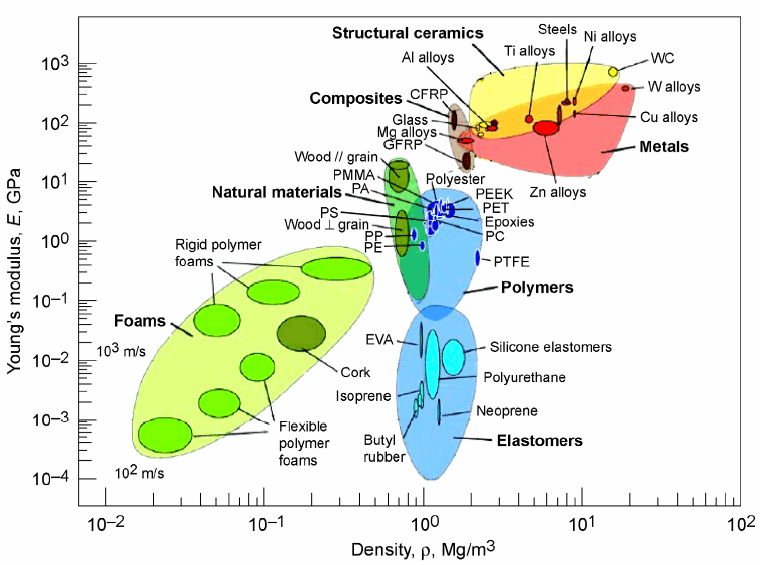
\includegraphics[width=0.75\textwidth]{figure11.png}%
\caption{Отношение вязкости разрушения от прочности для разнообразных материалов  (взято из \cite{ashby2005}). CFRP -- углепластик, DRA -- дискретно-армированный алюминий, GFRP -- стеклопластик, PA --- полианилин. PC--- поликарбон, PE --- полиэтилен, PMMA -- полиметилметакрилат (органическое стекло)}
\label{fig:figure11}
\end{figure}


Отметим, что композитные материалы, в целом, обеспечивают высокую вязкость разрушения наряду с низкой удельной плотностью, что делает их желательными для данного применения. Вязкость разрушения становится проблемой, особенно при криогенных температурах, когда многие материалы становятся чрезмерно хрупкими. Материалы с более высокой вязкостью разрушения желательны, поскольку они обеспечивают более устойчивые к повреждениям системы. Любая трещина, распространяющаяся в системе изоляции, может нарушить тепловые свойства системы изоляции -- что приведет к провалу миссии, поскольку произойдет быстрое выкипание криогенного топлива. На \cref{fig:figure11} представлен модуль Юнга E в зависимости от массовой плотности \(\rho\) для различных используемых материалов. Хотя это и не является основной переменной при проектировании, желательно выбрать жесткий материал, который минимизирует деформацию при нагрузках при сохранении низкой массы. Как и раньше, КПМ и металлические материалы обеспечивают желательную удельную жесткость для данного применения.



Анализируя рисунки \cref{fig:figure7}---\cref{fig:figure11}, можно сказать, что варианты материалов для стенки резервуара включают металлы, КПМ и металломатричные композиты (ММК). Композитные материалы могут также включать многослойную конструкцию, а также материалы, армированные наноразмерными частицами. Как отмечает Эсгар (\cite{esgar1962}), отношение прочности к плотности материала должно быть как можно выше, при этом материал должен иметь минимальные проблемы с изготовлением и не подвержен критическому хрупкому разрушению. Проникновение водорода в структуру резервуара должно быть сведено к минимуму. Металлы, обладающие приемлемыми свойствами от температуры окружающей среды до криогенных температур, включают аустенитные нержавеющие стали, монель и алюминиевые сплавы, как отмечает Рейнольдс (\cite{reynolds1955}). Кроме того, титан и медь обладают приемлемыми свойствами для криогенной эксплуатации, согласно Vance (\cite{vance1964}).

Имеется преимущество в использовании монолитного материала для создания резервуара, как в случаях, упомянутых выше выше. Использование одного материала для стенки резервуара устраняет термически индуцированные внутренние напряжения, вызванные различными КТР , таких как типичные составляющие материала КПМ или MMC. Однако, скорее всего, монолитные металлические резервуары будут не такими легкими, как их аналоги из КПМ или КДА. Металлическая структура подходит для наземных систем, где вес не является столь значительным ограничением, как для аэронавтики или систем космического базирования.

Композитные материалы, в частности КПМ, обладают меньшей плотностью и более высокой прочностью и жесткостью, чем металлы. используемых для криогенных задач. По оценкам, композиты могут обеспечить 25-процентную экономию веса по сравнению с новейшими монолитными алюминиевыми резервуарами в этом применении, как сообщает Sharke (\cite{sharke2004}).
Хотя смолы, используемые в полимерных матричных композитах, имеют склонность к более высокой проницаемости водорода. чем металлы. Брюер (\cite{brewer1991}) отметил, что традиционные композитные структуры с намотанными нитями традиционно не использовались для водородных резервуаров из-за диффузии водорода через промежутки в ив течение длительного времени. Однако разработка композитных баков началась в рамках программы NASP.  Робинсон и др. (\cite{robinson2002}) сообщили, что на основании результатов первоначальных исследований водородная проницаемость не является техническим препятствием для разработки композитного резервуара без вкалыдыша.

Материалы, которые подходят для применения в качестве стенок резервуара, включают монолитные металлы, непрерывно-армированные волокно армированные КПМ, и КДА. Это те классы материалов, которые должны быть дополнительно оценены основываясь на показателях эффективности, рассмотренные выше. Механические свойства, водородная проницаемость, технологичность и стоимость - это некоторые из прочих важных вопросов, которые следует рассмотреть для определения наиболее оптимальной системы материалов для строительства стенки резервуара.

\subsubsection{Особенности конструкции стенки резервуара}\label{ch:overview:1:sec4:sub2:subsub2}

Выбор материала для стенки резервуара -- это лишь один из важных вопросов в процессе проектирования. Геометрия стенки резервуара - еще один важный вопрос. В прошлом использовались различные конфигурации стенок резервуара.  Многие из предыдущих аэрокосмических применений были относительно краткосрочными. В результате одностенная конструкция с ребрами жесткости был распространен. В более поздних экспериментальных проектах использовались двустенные конструкции, включая композитные многослойные конструкции, но с газовой продувкой, а не с вакуумной оболочкой.

Схемы конструкции стенок требуют более глубокого исследования для определения оптимальной, легкой конструкции с соответствующим методом изоляции для удовлетворения потребностей применения в самолете. В \cref{tab:table6} кратко изложены преимущества и недостатки различных методов строительства стенок бака. Изгибающие напряжения в баке возникают в результате всплеска топлива и нагрузок, возникающих на опорных точках. Форма резервуара влияет на его способность выдерживать эти напряжения. Определенные геометрические формы, такие как сфера, могут минимизировать изгибающие напряжения в стенке резервуара. Таким образом, если резервуар должен быть изготовлен в виде цилиндрической конфигурации или более сложной правильной геометрии, то может оказаться полезным выбрать конструкцию стенки, способную выдерживать изгиб.

Две общие категории конструкции стенок резервуара - это одностенные и двустенные конструкции. В связи с необходимостью поддержания низкого теплового потока в течение длительного времени для данного применения используется изолирующая система, как обсуждалось в предыдущем разделе, скорее всего, будет состоять из высоковакуумной основы, что обуславливает использование двустенной конструкции резервуара.

Одностенные конструкции имеют преимущества относительно простой конструкции и низкой стоимости. Однако они могут использоваться только с изоляционной системой на основе пены или аналогичной, и поэтому вряд ли смогут удовлетворить требование низкого теплового потока сквозь стенку для применения в ЛА. Одностенная пенопластовая система вполне подходит для относительно краткосрочного применения, например, для космического челнока "space shuttle".

Двустенная конструкция, напротив, может представлять собой конструкцию типа "сэндвич" с несущей сердцевиной, которая выдерживает различные нагрузки. Кроме того, материал сердцевины может обладать изоляционными свойствами, что ограничивает тепловой поток в бак. В качестве альтернативы, в двустенной конструкции могут использоваться две структурные стенки с минимальным физическим контактом с высоковакуумной изоляционной системой.


\begin{table}
\centering
\small
\caption{Преимущества и недостатки различных конфигураций стенок резервуара для хранения жидкого водорода}
\label{tab:table6}
\begin{tabular}{|l|l|}
\hline
\multicolumn{2}{|c|}{\textbf{Одностенная конструкция}}                                                                                                                                                                                           \\ 
\hline
"+" & \begin{tabular}[c]{@{}l@{}}Простая конструкция\\Не дорогое производство\end{tabular}                                                                                                                                                        \\ 
\hline
"-" & \begin{tabular}[c]{@{}l@{}}Ограниченное количество схем изоляций\\Не оптимальная по весу конструкция\\Не практично при долгосрочном применении\end{tabular}                                                                                 \\ 
\hline
\multicolumn{2}{|c|}{\textbf{Двустенная конструкция}}                                                                                                                                                                                                     \\ 
\hline
"+" & \begin{tabular}[c]{@{}l@{}}Оптимальная по весу конструкция\\Больше схем изоляции\end{tabular}                                                                                                                                               \\ 
\hline
"-" & \begin{tabular}[c]{@{}l@{}}Высокая стоимость\\Сложное производство\end{tabular}                                                                                                                                                             \\ 
\hline
\multicolumn{2}{|c|}{\textbf{Постоянная толщина}}                                                                                                                                                                                                 \\ 
\hline
"+" & \begin{tabular}[c]{@{}l@{}}Простая конструкция\\Не дорогое производство\end{tabular}                                                                                                                                                        \\ 
\hline
"-" & \begin{tabular}[c]{@{}l@{}}Ограниченное количество схем изоляции\\Не оптимальная по весу конструкция\\Не оптимально при долгосрочном использовании\end{tabular}                                                                             \\ 
\hline
\multicolumn{2}{|c|}{\textbf{Переменная толщина (ребра жесткости)}}                                                                                                                                                                               \\ 
\hline
"+" & \begin{tabular}[c]{@{}l@{}}Легковесная конструкция\\Можно оптимизировать под конкретное применение\\Адаптируемые свойства\end{tabular}                                                                                                      \\ 
\hline
"-" & \begin{tabular}[c]{@{}l@{}}Сложное изготовлени\\Высокая стоимость\\Ограниченное количество схем изоляции\\Не оптимально при долгосрочном использовании\end{tabular}                                                                         \\ 
\hline
\multicolumn{2}{|c|}{\textbf{Стенка с наполнителем (сендвич)}}                                                                                                                                                                                    \\ 
\hline
"+" & \begin{tabular}[c]{@{}l@{}}Легковесная конструкция\\Хорошо подходит для нагрузок в плоскости и при изгибе\\Лучшие механическте свойства\\Наполнитель может иметь изоляционные свойства\end{tabular}                                         \\ 
\hline
"-" & \begin{tabular}[c]{@{}l@{}}Проблемы изготовления для больших конструкций (размер)\\Высокая цена\end{tabular}                                                                                                                                \\ 
\hline
\multicolumn{2}{|c|}{\textbf{Неструктурный наполнитель}}                                                                                                                                                                                          \\ 
\hline
"+" & \begin{tabular}[c]{@{}l@{}}Легковесный\\Хорошо подходит к экстремально низким температурам и вакууму\end{tabular}                                                                                                                           \\ 
\hline
"-" & \begin{tabular}[c]{@{}l@{}}Более толстые стенки, больший вес\\Сложность производства и стоимость\\Критически важным является поддержание высокого уровня вакуума,\\поэтому потеря вакуума приводит к катастрофическому отказу\end{tabular}  \\
\hline

\end{tabular}
\end{table}
